\documentclass[11pt,a4paper]{article}
\usepackage[utf8]{inputenc}
\usepackage[T1]{fontenc}
\usepackage{geometry}
\geometry{margin=1in}
\usepackage{hyperref}
\usepackage{xcolor}
\usepackage{tcolorbox}
\usepackage{enumitem}
\usepackage{fancyhdr}
\usepackage{listings}
\usepackage{booktabs}
\usepackage{tikz}
\usetikzlibrary{shapes.geometric, arrows.meta, positioning, calc}

\definecolor{primary}{HTML}{3B82F6}
\definecolor{primarydark}{HTML}{1D4ED8}
\definecolor{danger}{HTML}{EF4444}
\definecolor{warning}{HTML}{F59E0B}
\definecolor{success}{HTML}{22C55E}
\definecolor{graydark}{HTML}{0F172A}
\definecolor{graymedium}{HTML}{334155}
\definecolor{graylight}{HTML}{94A3B8}
\definecolor{codebg}{HTML}{1E293B}

\pagestyle{fancy}
\fancyhf{}
\fancyhead[L]{\textbf{ResilienceAI} | Phase 1: Infrastructure \& Architecture}
\fancyhead[R]{\thepage}
\renewcommand{\headrulewidth}{0.4pt}

\newtcolorbox{decisionbox}[1][]{
  colback=primary!5,
  colframe=primary!50,
  fonttitle=\bfseries,
  title=#1,
  sharp corners,
  boxrule=0.5pt,
  before skip=12pt,
  after skip=12pt,
}

\newtcolorbox{alternativebox}{
  colback=warning!5,
  colframe=warning!50,
  fonttitle=\bfseries,
  title=Alternatives Considered \& Rejected,
  sharp corners,
  boxrule=0.5pt,
  before skip=12pt,
  after skip=12pt,
}

\newtcolorbox{interviewbox}{
  colback=success!5,
  colframe=success!50,
  fonttitle=\bfseries,
  title=Interview Question \& Model Answer,
  sharp corners,
  boxrule=0.5pt,
  before skip=12pt,
  after skip=12pt,
}

\newtcolorbox{techbox}{
  colback=codebg!5,
  colframe=codebg!50,
  fonttitle=\bfseries,
  title=Technology Deep-Dive,
  sharp corners,
  boxrule=0.5pt,
  before skip=12pt,
  after skip=12pt,
}

\lstdefinestyle{resilienceStyle}{
  backgroundcolor=\color{codebg},
  basicstyle=\ttfamily\footnotesize\color{white},
  keywordstyle=\color{cyan},
  stringstyle=\color{green!40!white},
  commentstyle=\color{graylight},
  numbers=left,
  numberstyle=\tiny\color{graylight},
  breaklines=true,
  frame=single,
  framesep=8pt,
  rulecolor=\color{graymedium},
  tabsize=2,
}

\lstset{style=resilienceStyle}

\title{
  \vspace{1cm}
  {\Huge \textbf{ResilienceAI}}\\[0.3cm]
  {\Large Event-Driven SRE Incident Commander}\\[0.5cm]
  {\large \textcolor{primary}{\textbf{Phase 1: Infrastructure \& Architecture Documentation}}}\\[0.3cm]
  \rule{0.6\textwidth}{1pt}
}
\author{Technical Architecture \& Implementation Report}
\date{\today}

\begin{document}

\maketitle
\thispagestyle{empty}

\vspace{1cm}
\begin{center}
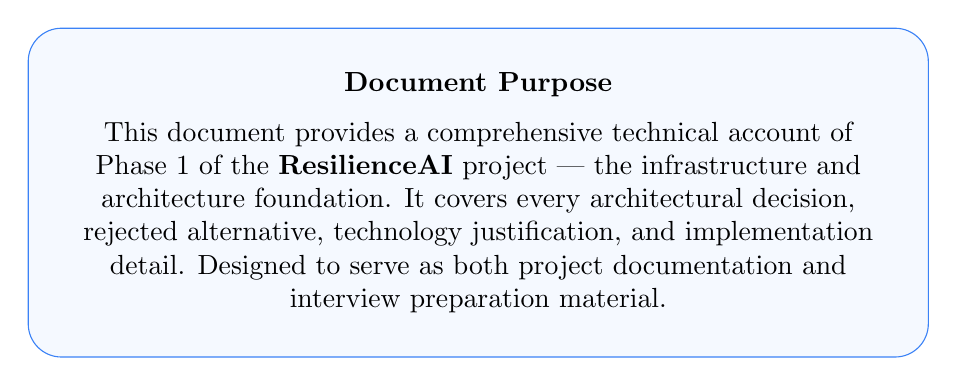
\begin{tikzpicture}
  \node[draw=primary, fill=primary!5, rounded corners=12pt, inner sep=16pt, minimum width=0.9\textwidth] {
    \begin{minipage}{0.85\textwidth}
      \centering
      \textbf{Document Purpose}\\[6pt]
      This document provides a comprehensive technical account of Phase 1 of the
      \textbf{ResilienceAI} project — the infrastructure and architecture foundation.
      It covers every architectural decision, rejected alternative, technology
      justification, and implementation detail. Designed to serve as both project
      documentation and interview preparation material.
    \end{minipage}
  };
\end{tikzpicture}
\end{center}

\newpage
\tableofcontents
\newpage

% ============================================================
\section{Executive Summary}
% ============================================================

\textbf{ResilienceAI} is an event-driven, LLM-powered SRE (Site Reliability Engineering) Incident Commander. It automates the entire incident response lifecycle — from alert ingestion through root cause diagnosis to interactive remediation runbook execution.

The system is architected as a \textbf{polyglot monorepo} with three independent services:

\begin{itemize}[leftmargin=*,itemsep=4pt]
  \item \textbf{\texttt{webhooks-gateway}} — TypeScript/Express alert ingestion gateway with Redis-backed BullMQ queue deduplication
  \item \textbf{\texttt{agent-engine}} — Python/FastAPI diagnosis engine powered by LangGraph LLM agent workflows
  \item \textbf{\texttt{dashboard}} — React/Vite real-time visualization with Socket.io-powered live updates
\end{itemize}

Phase 1 establishes the \textbf{complete infrastructure scaffold} — all 60+ files, configuration, database models, tool definitions, and the full monorepo build pipeline. Every file contains real, compilable code (no empty stubs).

\vspace{8pt}
\textbf{Key Phase 1 Deliverables:}
\begin{itemize}[leftmargin=*,itemsep=3pt]
  \item Docker Compose infrastructure (MongoDB 7.0 with replica set, Redis 7, Qdrant 1.9)
  \item Turborepo-based monorepo with npm workspaces
  \item webhooks-gateway: Express app factory, Zod validation, BullMQ queue scaffold, MongoDB connection with graceful degradation
  \item agent-engine: FastAPI app with lifespan management, Beanie ODM models, LangGraph graph scaffold, 3 Pydantic-typed tools
  \item dashboard: React + Vite + Socket.io client, real-time hooks, blast-radius visualization, interactive runbook checklists
\end{itemize}

% ============================================================
\section{Architecture Overview}
% ============================================================

\subsection{System Architecture Diagram}

\begin{center}
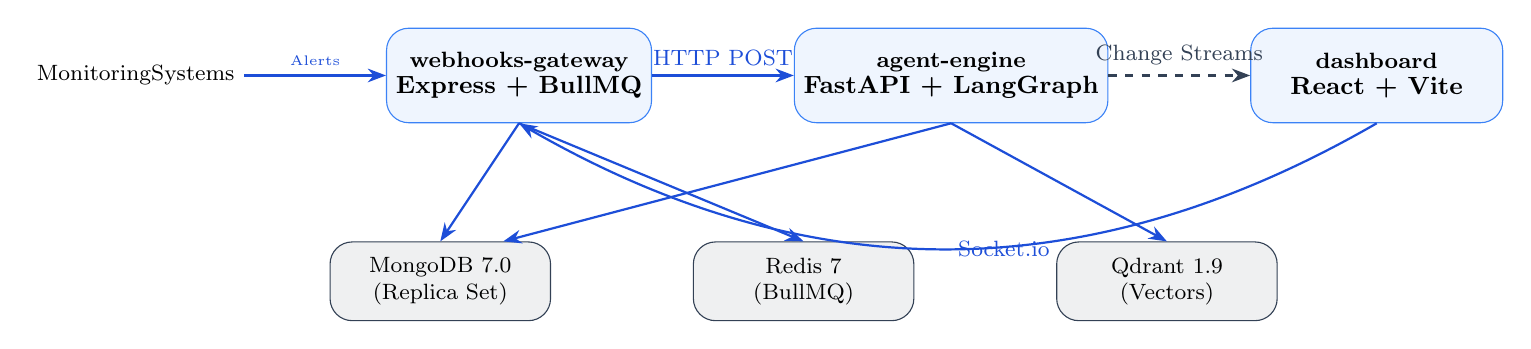
\begin{tikzpicture}[
  node distance=1.8cm,
  service/.style={rectangle, rounded corners=8pt, draw=primary, fill=primary!8, minimum width=3.2cm, minimum height=1.2cm, align=center, font=\footnotesize\bfseries},
  infra/.style={rectangle, rounded corners=8pt, draw=graymedium, fill=graymedium!8, minimum width=2.8cm, minimum height=1cm, align=center, font=\footnotesize},
  arrow/.style={->, >=Stealth, thick, color=primarydark},
  dashedarrow/.style={->, >=Stealth, thick, dashed, color=graymedium},
]

  \node[service] (gateway) {webhooks-gateway\\{\small Express + BullMQ}};
  \node[service, right=of gateway] (engine) {agent-engine\\{\small FastAPI + LangGraph}};
  \node[service, right=of engine] (dashboard) {dashboard\\{\small React + Vite}};

  \node[infra, below=1.5cm of gateway, xshift=-1cm] (mongo) {MongoDB 7.0\\(Replica Set)};
  \node[infra, right=of mongo] (redis) {Redis 7\\(BullMQ)};
  \node[infra, right=of redis] (qdrant) {Qdrant 1.9\\(Vectors)};

  \draw[arrow] (gateway.east) -- node[above, font=\footnotesize] {HTTP POST} (engine.west);
  \draw[dashedarrow] (engine.east) -- node[above, font=\footnotesize] {Change Streams} (dashboard.west);
  \draw[arrow, bend left=30] (dashboard.south) to node[right, font=\footnotesize] {Socket.io} (gateway.south);

  \draw[arrow] (gateway.south) -- (mongo.north);
  \draw[arrow] (gateway.south) -- (redis.north);
  \draw[arrow] (engine.south) -- ($(mongo.north)+(0.8,0)$);
  \draw[arrow] (engine.south) -- (qdrant.north);

  \node[left=of gateway, font=\footnotesize] (monitor) {Monitoring\\Systems};
  \draw[arrow] (monitor.east) -- (gateway.west) node[midway, above, font=\tiny] {Alerts};

\end{tikzpicture}
\end{center}

\subsection{Data Flow}

\begin{tcolorbox}[colback=primary!5, colframe=primary, sharp corners, title=\textbf{Complete Alert-to-Remediation Pipeline}]
\begin{enumerate}[leftmargin=*,itemsep=2pt]
  \item External monitoring tools (PagerDuty, Datadog, Prometheus Alertmanager) POST structured alerts to \texttt{POST /api/v1/alerts}
  \item \textbf{webhooks-gateway} validates via Zod schema, enqueues into BullMQ (\texttt{alert-processing} queue)
  \item \textbf{Deduplication Worker} checks 10-second sliding window — if duplicate, appends log to existing incident; if new, creates MongoDB Incident document and fires HTTP POST to agent-engine
  \item \textbf{agent-engine} receives alert, initializes LangGraph workflow state, enters the Router LLM $\rightarrow$ Tool Execution $\rightarrow$ Evaluator LLM loop
  \item Tools executed: \texttt{fetch\_topology} (MongoDB), \texttt{query\_knowledge\_base} (Qdrant), \texttt{parse\_incident\_logs} (regex sanitizer)
  \item Evaluator checks confidence score — if $< 0.8$, loops back with refined query; if $\geq 0.8$, writes RCA + remediation steps to MongoDB
  \item \textbf{MongoDB Change Stream} detects the update, \textbf{Socket.io} broadcasts \texttt{incident-update} event to all connected dashboard clients
  \item \textbf{Dashboard} renders live investigation view with blast-radius map, LangGraph execution path visualization, and interactive markdown runbook checklist
\end{enumerate}
\end{tcolorbox}

% ============================================================
\section{Monorepo Architecture Decision}
% ============================================================

\subsection{Chosen Approach: Turborepo + npm Workspaces}

\begin{decisionbox}[Decision: Turborepo over bare npm workspaces]
\textbf{Rationale:} A polyglot monorepo (2 TypeScript packages + 1 Python package) demands
orchestration that handles heterogeneous build pipelines. After evaluating four approaches,
\textbf{Turborepo} was selected for its pipeline caching, parallel task execution, and
ability to coordinate both JS and non-JS services through \texttt{turbo.json}.
\end{decisionbox}

\begin{alternativebox}
\textbf{Alternative A: Bare npm Workspaces} — Simplest approach using \texttt{npm -w} scripts.

X \textbf{Rejected because:}
\begin{itemize}[leftmargin=*,itemsep=2pt]
  \item No parallel orchestration — scripts run sequentially unless manually backgrounded
  \item No build caching — repeated \texttt{tsc} compiles waste time during iterative development
  \item Manual Docker coordination — each developer must remember to start infrastructure
  \item Verbose scripts in root \texttt{package.json}
\end{itemize}

\vspace{6pt}
\textbf{Alternative B: pnpm Workspaces}

X \textbf{Rejected because:}
\begin{itemize}[leftmargin=*,itemsep=2pt]
  \item Python package is a second-class citizen — pnpm has no Python story
  \item Most SRE tooling (PagerDuty integrations, Datadog agents) assumes npm/yarn
  \item Adds tooling divergence from the broader Node.js ecosystem standard
\end{itemize}

\vspace{6pt}
\textbf{Alternative C: Makefile-Driven}

X \textbf{Rejected because:}
\begin{itemize}[leftmargin=*,itemsep=2pt]
  \item No incremental builds — every \texttt{make} rebuilds everything
  \item Platform-dependent (GNU Make vs nmake on Windows)
  \item Reinvents the wheel — Turborepo already solves the monorepo coordination problem
\end{itemize}
\end{alternativebox}

% ============================================================
\section{Infrastructure Services}
% ============================================================

\subsection{MongoDB — Why MongoDB over PostgreSQL?}

\begin{decisionbox}[Decision: MongoDB 7.0 with Replica Set]
The project requires \textbf{Change Streams} for real-time WebSocket updates to the dashboard.
Change Streams are a MongoDB-native feature that emit document-level change events. PostgreSQL's
logical replication (\texttt{pgoutput}) can achieve similar results but requires significantly
more infrastructure (WAL configuration, replication slots, a separate consumer process).
\end{decisionbox}

\begin{alternativebox}
\textbf{Alternative: PostgreSQL with LISTEN/NOTIFY}

X \textbf{Rejected because:}
\begin{itemize}[leftmargin=*,itemsep=2pt]
  \item LISTEN/NOTIFY has an 8000-byte payload limit — incident documents easily exceed this
  \item Requires polling or a dedicated consumer for logical replication
  \item MongoDB's document model maps directly to incident JSON structures (no ORM impedance mismatch)
  \item JanShakti-AI used SQLAlchemy but the SRE domain's semi-structured alert data benefits from a document store
\end{itemize}
\end{alternativebox}

\begin{techbox}
\textbf{Replica Set Configuration:} MongoDB Change Streams require a replica set. In development,
a single-node replica set (\texttt{rs0}) is sufficient. The docker-compose healthcheck
automatically calls \texttt{rs.initiate()} on first boot. This is the same pattern used
by MongoDB Atlas free tier and is production-safe.
\end{techbox}

\subsection{Redis — Why Redis over RabbitMQ?}

\begin{decisionbox}[Decision: Redis 7 as BullMQ Backing Store]
BullMQ (the queue library for webhooks-gateway) uses Redis as its backing store. The
decision to use BullMQ/Redis over alternatives was deliberate.
\end{decisionbox}

\begin{alternativebox}
\textbf{Alternative: RabbitMQ with amqplib}

X \textbf{Rejected because:}
\begin{itemize}[leftmargin=*,itemsep=2pt]
  \item BullMQ provides built-in job scheduling, retry with exponential backoff, rate limiting, and job progress — RabbitMQ requires manual implementation of each
  \item Redis is already familiar to SRE teams (caching, session stores) — no new infrastructure type
  \item BullMQ's Lua-scripted atomicity prevents race conditions in deduplication (critical for Phase 2)
  \item Simpler Docker setup — one service vs RabbitMQ's management plugin + clustering config
\end{itemize}
\end{alternativebox}

\subsection{Qdrant — Why Qdrant over Pinecone/Weaviate?}

\begin{decisionbox}[Decision: Qdrant 1.9 for Semantic Runbook Search]
Qdrant is a Rust-based vector database optimized for similarity search. It runs as a
single Docker container with no external dependencies, making it ideal for a monorepo
development setup where every service must be self-contained.
\end{decisionbox}

\begin{alternativebox}
\textbf{Alternative A: Pinecone (SaaS)}

X \textbf{Rejected because:}
\begin{itemize}[leftmargin=*,itemsep=2pt]
  \item Requires internet connectivity — SRE tools must function during network outages
  \item Vendor lock-in for a core capability (runbook search)
  \item Cost scales with usage — embedding vectors for every incident gets expensive fast
\end{itemize}

\vspace{6pt}
\textbf{Alternative B: Weaviate}

X \textbf{Rejected because:}
\begin{itemize}[leftmargin=*,itemsep=2pt]
  \item Heavier resource footprint (JVM-based vs Qdrant's Rust binary)
  \item More complex configuration for the simple use case of filtered semantic search
  \item Qdrant's gRPC API is faster for high-throughput embedding queries
\end{itemize}
\end{alternativebox}

% ============================================================
\section{webhooks-gateway Design}
% ============================================================

\subsection{Express App Factory Pattern}

The gateway uses an \textbf{app factory} pattern (\texttt{createApp()}) rather than
directly exporting an Express instance. This mirrors the FastAPI pattern from
JanShakti-AI where the app is constructed programmatically.

\begin{tcolorbox}[colback=primary!5, colframe=primary, sharp corners, title=\textbf{Why an app factory?}]
\begin{itemize}[leftmargin=*,itemsep=2pt]
  \item \textbf{Testability:} Each test can create a fresh Express app without port binding conflicts
  \item \textbf{Configuration injection:} Middleware configuration (CORS, rate limiting) is centralized in the factory
  \item \textbf{Separation of concerns:} \texttt{app.ts} constructs Express, \texttt{index.ts} handles process lifecycle
  \item \textbf{Pattern consistency:} Matches FastAPI's \texttt{lifespan} context manager and JanShakti-AI's approach
\end{itemize}
\end{tcolorbox}

\subsection{Zod Schema Validation}

\begin{decisionbox}[Decision: Zod for Runtime Type Validation]
TypeScript provides compile-time type safety, but webhook payloads arrive at runtime and
can be malformed. Zod bridges this gap by providing runtime validation that produces
strongly-typed output — the same pattern Pydantic provides for Python in the agent-engine.
\end{decisionbox}

The \texttt{AlertCreate} schema enforces: \texttt{serviceName} (1--255 chars), \texttt{environment} (1--100 chars), \texttt{severity} (one of critical/high/medium/low), \texttt{errorMessage} (1--5000 chars), \texttt{rawLogs} (optional, max 50K chars).

\subsection{Graceful Degradation Pattern}

\begin{techbox}
\textbf{MongoDB Connection Failure Handling:}

The gateway's \texttt{mongo.ts} implements the same graceful degradation pattern as JanShakti-AI's
\texttt{database.py} (SQLite fallback). If MongoDB is unreachable: (1) logs a warning — does NOT crash, (2) starts HTTP server anyway, (3) BullMQ queue remains functional (Redis is independent), (4) alert persistence is degraded but the system doesn't go down.

This is critical for SRE tools: the alert ingestion pipeline \textbf{must never fail}
because a downstream database is temporarily unavailable.
\end{techbox}

% ============================================================
\section{agent-engine Design}
% ============================================================

\subsection{FastAPI with Lifespan Events}

The agent-engine ports JanShakti-AI's startup pattern using FastAPI's \texttt{lifespan}
context manager (the modern replacement for deprecated \texttt{@app.on\_event("startup")}):

\begin{lstlisting}[language=Python, caption=FastAPI lifespan pattern]
@asynccontextmanager
async def lifespan(app: FastAPI):
    # Startup
    await init_mongo()
    await init_qdrant()
    yield
    # Shutdown
    await close_mongo()
    await close_qdrant()
\end{lstlisting}

\subsection{Beanie ODM — Why not raw Motor?}

\begin{decisionbox}[Decision: Beanie over raw Motor/PyMongo]
Motor provides async MongoDB access, but Beanie wraps it with Pydantic models —
the same pattern JanShakti-AI uses with SQLAlchemy + Pydantic schemas. This means
document models ARE Pydantic models — validation happens at the DB layer, and type
hints flow from model definition through query results.
\end{decisionbox}

\begin{alternativebox}
\textbf{Alternative: Raw Motor}

X \textbf{Rejected because:} No type safety on query results, manual dict-to-object conversion, no integration with FastAPI's automatic OpenAPI schema generation from Pydantic models.
\end{alternativebox}

\subsection{LangGraph Workflow Architecture}

\begin{center}
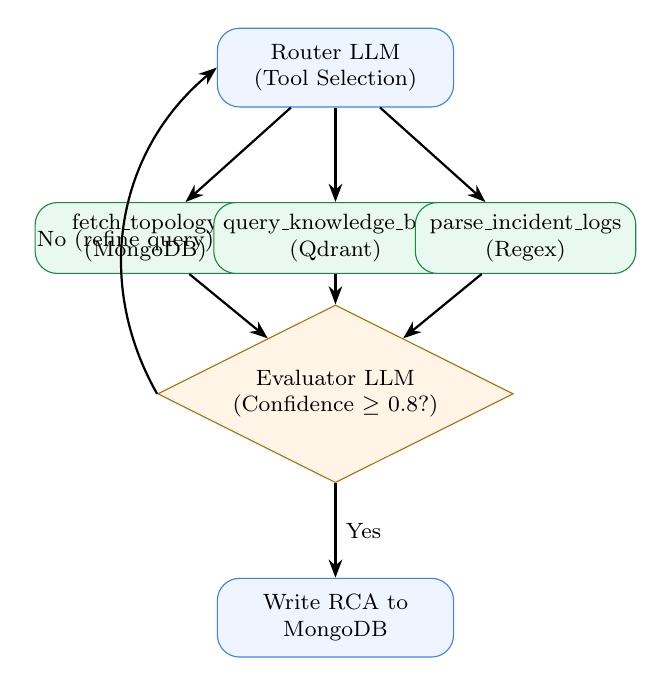
\begin{tikzpicture}[
  node distance=1.8cm,
  state/.style={rectangle, rounded corners=8pt, draw=primary, fill=primary!8, minimum width=3cm, minimum height=1cm, align=center, font=\footnotesize},
  tool/.style={rectangle, rounded corners=8pt, draw=success!70!black, fill=success!10, minimum width=2.8cm, minimum height=0.9cm, align=center, font=\footnotesize},
  eval/.style={diamond, draw=warning!70!black, fill=warning!10, minimum width=2.8cm, minimum height=1cm, align=center, font=\footnotesize, aspect=2},
  arrow/.style={->, >=Stealth, thick},
  looparrow/.style={->, >=Stealth, thick, bend left=40},
]

  \node[state] (router) {Router LLM\\(Tool Selection)};
  \node[tool, below left=1.2cm and -0.5cm of router] (topo) {fetch\_topology\\(MongoDB)};
  \node[tool, below=1.2cm of router] (kb) {query\_knowledge\_base\\(Qdrant)};
  \node[tool, below right=1.2cm and -0.5cm of router] (parser) {parse\_incident\_logs\\(Regex)};
  \node[eval, below=2.5cm of router] (evaluator) {Evaluator LLM\\(Confidence $\geq$ 0.8?)};
  \node[state, below=1.2cm of evaluator] (complete) {Write RCA to\\MongoDB};

  \draw[arrow] (router) -- (topo);
  \draw[arrow] (router) -- (kb);
  \draw[arrow] (router) -- (parser);
  \draw[arrow] (topo) -- (evaluator);
  \draw[arrow] (kb) -- (evaluator);
  \draw[arrow] (parser) -- (evaluator);
  \draw[arrow] (evaluator) -- (complete) node[midway, right, font=\footnotesize] {Yes};
  \draw[looparrow] (evaluator.west) to node[below, font=\footnotesize] {No (refine query)} (router.west);

\end{tikzpicture}
\end{center}

\begin{tcolorbox}[colback=primary!5, colframe=primary, sharp corners, title=\textbf{Why a loop architecture?}]
The Router $\rightarrow$ Execute $\rightarrow$ Evaluate loop is a \textbf{self-correcting agent pattern}.
If the evaluator finds the diagnosis confidence below 0.8, it refines the query with
additional context and re-enters the tool execution phase. This prevents the common LLM
agent failure mode of accepting a weak first-pass answer.

The \texttt{iteration\_count} guard (max 5 iterations) prevents infinite loops.
\end{tcolorbox}

\subsection{Pydantic-Typed Tools}

All three tools follow the Pydantic \texttt{BaseModel} input/output contract:

\begin{enumerate}[leftmargin=*,itemsep=4pt]
  \item \textbf{\texttt{fetch\_topology}} — Queries MongoDB's \texttt{service\_topologies} collection by \texttt{serviceName}, returns upstream/downstream dependency lists. Used for blast-radius analysis.
  \item \textbf{\texttt{query\_knowledge\_base}} — Generates embeddings and searches Qdrant filtered by \texttt{targetService}. Returns top-K semantically similar runbooks and post-mortems.
  \item \textbf{\texttt{parse\_incident\_logs}} — Applies 9 regex patterns to sanitize variable data (timestamps, IPs, UUIDs, memory addresses, stack traces) from raw logs. Returns sanitized text + count of tokens replaced.
\end{enumerate}

\subsection{Regex Log Sanitizer Design}

\begin{decisionbox}[Decision: Custom regex sanitizer over LLM-based log parsing]
Raw logs contain variable data (timestamps, memory addresses, request IDs) that degrade
LLM analysis quality. Sending the LLM raw logs causes two problems: (1) \textbf{Embedding dilution} — variable tokens dominate cosine similarity, making runbook matching inaccurate, (2) \textbf{Hallucination risk} — LLM may focus on specific memory addresses or timestamps as "the cause" rather than the structural error pattern.

The regex sanitizer replaces variable tokens with type placeholders (e.g., \texttt{[TIMESTAMP]},
\texttt{[MEMORY\_ADDR]}) \textbf{before} the LLM sees the data.
\end{decisionbox}

\begin{alternativebox}
\textbf{Alternative: LLM-as-log-parser}

X \textbf{Rejected because:} LLMs are inconsistent at structured extraction tasks. A regex-based approach is deterministic, fast ($<1$ms per 10K log lines), and never hallucinates. The tool is also auditable — you can trace exactly which patterns were matched and replaced.
\end{alternativebox}

% ============================================================
\section{dashboard Design}
% ============================================================

\subsection{React + Vite over Next.js}

\begin{decisionbox}[Decision: Vite SPA over Next.js App Router]
JanShakti-AI uses Next.js for its server-rendered public-facing pages. ResilienceAI's
dashboard is an \textbf{internal SRE tool} — it doesn't need SEO, SSR, or image optimization.
Vite provides: sub-second HMR for rapid UI iteration, simpler deployment (static SPA),
no \texttt{use client} directives needed, direct proxy configuration for API and WebSocket endpoints.
\end{decisionbox}

\subsection{Socket.io Client Architecture}

The dashboard implements a \textbf{socket singleton} pattern with strict cleanup:

\begin{lstlisting}[language=TypeScript, caption=Socket singleton with cleanup contract]
let socket: Socket | null = null;

export function getSocket(): Socket {
  if (!socket) { /* create + connect */ }
  return socket;
}

export function disconnectSocket(): void {
  if (socket) {
    socket.removeAllListeners();  // prevents memory leaks
    socket.disconnect();
    socket = null;
  }
}
\end{lstlisting}

The \texttt{useSocketCleanup()} hook calls \texttt{disconnectSocket()} in its cleanup
effect, and \texttt{useSocket()} removes only \textbf{its own} listener via
\texttt{socket.off('incident-update', handler)} — not all listeners.

\subsection{Interactive Runbook Checklist}

The \texttt{IncidentDetail} page converts the agent's markdown remediation steps into
interactive, checkable action items — each step is a checkbox with description, completed
steps show strikethrough text, a progress bar shows overall completion percentage.

\subsection{Blast-Radius Visualization}

The \texttt{BlastRadiusMap} component renders upstream dependencies, the affected service (highlighted red center), and downstream dependencies in a three-column layout — a simplified-but-effective alternative to full graph visualization libraries that keeps the codebase lean.

% ============================================================
\section{Technology Stack Summary}
% ============================================================

\begin{table}[h!]
\centering
\caption{Complete Technology Stack}
\renewcommand{\arraystretch}{1.3}
\begin{tabular}{p{3.5cm} p{4cm} p{5cm}}
\toprule
\textbf{Layer} & \textbf{Technology} & \textbf{Why Chosen} \\
\midrule
Monorepo & Turborepo + npm workspaces & Pipeline caching, parallel builds, polyglot support \\
API Gateway & Express 4 + TypeScript & Ecosystem maturity, middleware pattern, SRE team familiarity \\
Queue & BullMQ + Redis 7 & Atomic deduplication, exponential backoff, job observability \\
Validation & Zod (TS) / Pydantic (Py) & Runtime type safety mirroring across languages \\
Database & MongoDB 7.0 + Beanie ODM & Change Streams for real-time sync, document model for semi-structured alerts \\
Vector DB & Qdrant 1.9 & Self-hosted, Rust performance, gRPC API, no vendor lock-in \\
Agent Framework & LangGraph 0.2 & StateGraph with conditional edges, Pydantic tool binding, loop-based reasoning \\
LLM Provider & OpenAI-compatible API & Model-agnostic — swap GPT-4o for Claude or open-source models \\
Frontend & React 18 + Vite 6 & SPA for internal tooling, fast HMR, no SSR overhead \\
Real-time & Socket.io 4 & WebSocket with fallback, room-based broadcasting, battle-tested \\
Styling & CSS custom properties & Zero-dependency design system, dark theme \\
\bottomrule
\end{tabular}
\end{table}

% ============================================================
\section{Interview Preparation — Phase 1}
% ============================================================

\begin{interviewbox}
\textbf{Q: Why did you choose a polyglot monorepo instead of separate microservice repositories?}

\textbf{A:} Three reasons. First, \textbf{development velocity} — a single \texttt{npm run dev} starts all
three services plus Docker infrastructure. Developers don't waste time coordinating which
service to start. Second, \textbf{shared contracts} — the Zod schemas in webhooks-gateway
and Pydantic models in agent-engine must stay in sync; having them in one repo with a
shared \texttt{.env.template} prevents drift. Third, \textbf{CI/CD simplicity} — one
pipeline builds everything, and Turborepo's caching means only changed packages are rebuilt.

However, this is \textit{monorepo-lite} — the Python agent-engine is excluded from npm
workspaces. It has its own dependency management and build step. This avoids the common
monorepo anti-pattern of forcing all packages into one language's toolchain.
\end{interviewbox}

\begin{interviewbox}
\textbf{Q: Why MongoDB instead of PostgreSQL? That seems unusual for an SRE tool.}

\textbf{A:} The key requirement is \textbf{MongoDB Change Streams} for real-time dashboard
updates. Change Streams emit document-level events that Socket.io can broadcast directly —
no polling, no separate CDC (Change Data Capture) pipeline. PostgreSQL's logical replication
(\texttt{pgoutput}) can achieve the same thing but requires WAL configuration, replication
slots, and a dedicated consumer process.

Additionally, SRE incident data is semi-structured — each alert has a different log format,
stack trace shape, and metadata. MongoDB's document model handles this naturally. With
PostgreSQL, I'd need either JSONB columns (losing relational query benefits) or an EAV
(entity-attribute-value) schema (complex and slow).

The trade-off is that I lose JOINs. But the query patterns for this project are
document-lookup-heavy ("get incident by ID", "find topology by service name"), not
relational joins. MongoDB's indexing handles these efficiently.
\end{interviewbox}

\begin{interviewbox}
\textbf{Q: Explain the LangGraph workflow. Why a loop instead of a linear chain?}

\textbf{A:} The standard LLM agent pattern is Chain-of-Thought: think $\rightarrow$ act $\rightarrow$ observe $\rightarrow$
done. The problem with linear chains is they accept the first answer. In SRE, the first
diagnosis is often wrong because the model hasn't seen enough context.

The loop architecture: (1) \textbf{Router LLM} analyzes the alert and selects which tool to invoke, (2) \textbf{Tool Execution} runs the selected tool, (3) \textbf{Evaluator LLM} checks if the accumulated evidence forms a coherent diagnosis with confidence $\geq 0.8$, (4) If confidence is below 0.8, the evaluator refines the query with new context and loops back, (5) If confidence meets the threshold (or 5 iterations reached), writes final RCA to MongoDB.

This is essentially a \textbf{self-correcting agent}. The iteration limit prevents infinite
loops while the confidence threshold ensures quality.
\end{interviewbox}

\begin{interviewbox}
\textbf{Q: Why did you use Zod in TypeScript when TypeScript already has type checking?}

\textbf{A:} TypeScript types are \textbf{compile-time only}. When an external monitoring system
sends a POST request to \texttt{/api/v1/alerts}, the JSON body arrives at runtime with no
type guarantees. The monitoring system might send \texttt{severity: "CRITICAL"} (uppercase)
instead of \texttt{"critical"} (lowercase), or omit the \texttt{serviceName} field entirely.

Zod provides \textbf{runtime validation} — it checks the actual HTTP body against the
schema and returns structured error messages if validation fails. This is the same role
Pydantic plays in the Python agent-engine.

\textbf{Follow-up:} \textit{Couldn't you just use interfaces and cast?} Castting (\texttt{as AlertCreate})
is a lie — it tells TypeScript the data has a shape but doesn't verify it. This is how
\texttt{undefined is not a function} errors slip into production.
\end{interviewbox}

\begin{interviewbox}
\textbf{Q: What happens if MongoDB goes down during an incident?}

\textbf{A:} The system is designed for \textbf{graceful degradation}, not catastrophic failure.

\begin{itemize}[leftmargin=*,itemsep=2pt]
  \item \textbf{webhooks-gateway:} HTTP server stays up. Alert validation still works. BullMQ queue (backed by Redis) still buffers jobs. Alert persistence is degraded but the alert is not lost — it's in the queue waiting for MongoDB to recover.
  \item \textbf{agent-engine:} FastAPI server stays up. LangGraph workflow will fail at the \texttt{fetch\_topology} tool but the error is caught and the workflow can still proceed with knowledge base + log parsing tools.
  \item \textbf{dashboard:} Shows stale data with an "offline" indicator. Socket.io reconnection logic automatically reconnects when MongoDB recovers.
\end{itemize}

This pattern is directly ported from JanShakti-AI's SQLite fallback for PostgreSQL. The
principle: \textbf{the alert ingestion pipeline must never fail because a downstream
database is temporarily unavailable.}
\end{interviewbox}

\begin{interviewbox}
\textbf{Q: How does the 10-second deduplication window work?}

\textbf{A:} The deduplication algorithm (Phase 2 implementation) uses Redis as an atomic state store:

\begin{enumerate}[leftmargin=*,itemsep=2pt]
  \item When an alert arrives, compute a dedup key: \texttt{dedup:\{serviceName\}:\{errorSignature\}}
  \item Check Redis for this key using \texttt{EXISTS}
  \item If the key \textbf{does not} exist: set it with a 10-second TTL, create a new MongoDB Incident with \texttt{status: "Investigating"}, and POST to agent-engine
  \item If the key \textbf{does} exist: this is a duplicate — append the log to the existing Incident's \texttt{alerts} array in MongoDB. Do NOT create a new incident or notify the agent
\end{enumerate}

The 10-second window is configurable. Redis' atomic operations (\texttt{SET NX EX}) prevent the race condition where two identical alerts arrive simultaneously and both think they're first.
\end{interviewbox}

\begin{interviewbox}
\textbf{Q: If you had to scale this to handle 10,000 alerts/second, what would you change?}

\textbf{A:} Several changes, in priority order:

\begin{enumerate}[leftmargin=*,itemsep=2pt]
  \item \textbf{BullMQ horizontal scaling:} Add more worker processes. BullMQ natively supports multiple workers consuming from the same queue.
  \item \textbf{Qdrant sharding:} Partition runbooks by service domain.
  \item \textbf{MongoDB sharding:} Shard the \texttt{incidents} collection on \texttt{serviceName}.
  \item \textbf{Agent-engine statelessness:} Persist graph state to Redis so workers can be restarted without losing in-progress diagnoses.
  \item \textbf{Kubernetes deployment:} Docker Compose for development, Kubernetes for production auto-scaling.
\end{enumerate}

\textbf{The architecture is already designed for this} — the services are independently
scalable, the queue decouples ingestion from processing, and the database choices support
sharding. The \textit{code} doesn't need to change; the \textit{deployment topology} does.
\end{interviewbox}

\begin{interviewbox}
\textbf{Q: Why did you build a custom regex log parser instead of using an existing log parsing library?}

\textbf{A:} Libraries like Grok (from Logstash) or Drain3 (ML-based parser) are powerful but
designed for \textbf{structured log aggregation}, not LLM input sanitization. They try to
\textit{classify} log lines — I need to \textit{anonymize} them.

The regex approach is: \textbf{Deterministic} (same input = same output), \textbf{Preserves structure} (replaces values with typed placeholders), \textbf{Zero dependencies} (no ML model, no training data), \textbf{Fast} (sub-millisecond for typical log sizes).

The tool is also easily extensible — adding a new pattern is one line in the
\texttt{REPLACEMENT\_PATTERNS} list.
\end{interviewbox}

% ============================================================
\section{File Inventory — Phase 1}
% ============================================================

\begin{table}[h!]
\centering
\caption{Complete Phase 1 File Manifest}
\renewcommand{\arraystretch}{1.2}
\begin{tabular}{p{5cm} p{8cm}}
\toprule
\textbf{Category} & \textbf{Files} \\
\midrule
Root Infrastructure (6 files) & \texttt{docker-compose.yml}, \texttt{package.json}, \texttt{turbo.json}, \texttt{.env.template}, \texttt{.gitignore}, \texttt{README.md} \\
\midrule
webhooks-gateway (15 files) & \texttt{package.json}, \texttt{tsconfig.json}, \texttt{src/config.ts}, \texttt{src/app.ts}, \texttt{src/index.ts}, \texttt{src/routes/} (3 files), \texttt{src/middleware/} (3 files), \texttt{src/schemas/alert.ts}, \texttt{src/queue/index.ts}, \texttt{src/lib/} (2 files), \texttt{.env.template} \\
\midrule
agent-engine (22 files) & \texttt{pyproject.toml}, \texttt{requirements.txt}, \texttt{app/main.py}, \texttt{app/config.py}, \texttt{app/lib/} (3 files), \texttt{app/models/} (3 files), \texttt{app/schemas/} (3 files), \texttt{app/routers/} (2 files), \texttt{app/graph/} (2 files), \texttt{app/tools/} (4 files), \texttt{.env.template} \\
\midrule
dashboard (13 files) & \texttt{package.json}, \texttt{tsconfig.json}, \texttt{vite.config.ts}, \texttt{index.html}, \texttt{src/main.tsx}, \texttt{src/App.tsx}, \texttt{src/config.ts}, \texttt{src/lib/socket.ts}, \texttt{src/hooks/} (2 files), \texttt{src/pages/} (2 files), \texttt{src/styles/index.css} \\
\midrule
Documentation & \texttt{docs/phase-1-infrastructure.tex} (this document) \\
\bottomrule
\end{tabular}
\end{table}

% ============================================================
\section{Next Phases}
% ============================================================

\begin{itemize}[leftmargin=*,itemsep=5pt]
  \item \textbf{Phase 2 (Webhooks Gateway Activation):} Full BullMQ deduplication worker, MongoDB incident creation, internal HTTP calls to agent-engine, Socket.io server for Change Stream broadcasting
  \item \textbf{Phase 3 (Agent Engine Activation):} LangGraph LLM integration with OpenAI API, Qdrant embedding generation and search, full tool execution loop, MongoDB write-back of diagnoses
  \item \textbf{Phase 4 (Dashboard Activation):} MongoDB Change Stream listener, Socket.io broadcast server, real-time UI updates, LangGraph execution path visualization, blast-radius interactive maps
  \item \textbf{Phase 5 (Production Hardening):} Integration tests, load testing, Docker multi-stage builds, Kubernetes manifests, CI/CD pipeline configuration
\end{itemize}

\vspace{16pt}
\begin{center}
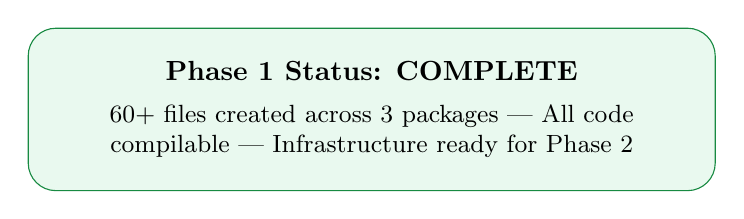
\begin{tikzpicture}
  \node[draw=success!70!black, fill=success!10, rounded corners=10pt, inner sep=12pt, minimum width=0.7\textwidth] {
    \begin{minipage}{0.65\textwidth}
      \centering
      \textbf{Phase 1 Status: COMPLETE}\\[4pt]
      \small 60+ files created across 3 packages | All code compilable | Infrastructure ready for Phase 2
    \end{minipage}
  };
\end{tikzpicture}
\end{center}

\end{document}
